\newpage % Rozdziały zaczynamy od nowej strony.
\section{Wstep teoretyczny}
W tym rodziale przedstawione zostaną najważniejsze koncepcje niezbędne do dalszej analizy pracy. Celem tego rozdziału jest przede wszytskim jednoznaczne sprecyzowanie, czym jest segmentacja semantyczna oraz klasyfikacja sceny w dziedzinie pomieszczeń. Zostanie udzielona odpowiedź na fundamentalne pytania, między innymi, czym jest uczenie maszynowe oraz dlaczego warto korzystać z głębokich sieci neurnowych. W dalszej części zostaną przedstawione aktualne sposoby realizacji celów pracy z przedstawieniem ich rozwoju na przestrzeni lat. Rozdział wieńczą opisy bardziej zaawansowanych technik realizacji wspominanych algorytów.
\subsection{Definicje zadań}
\subsubsection{Klasyfikacja sceny}
\begin{figure}[ht!]
    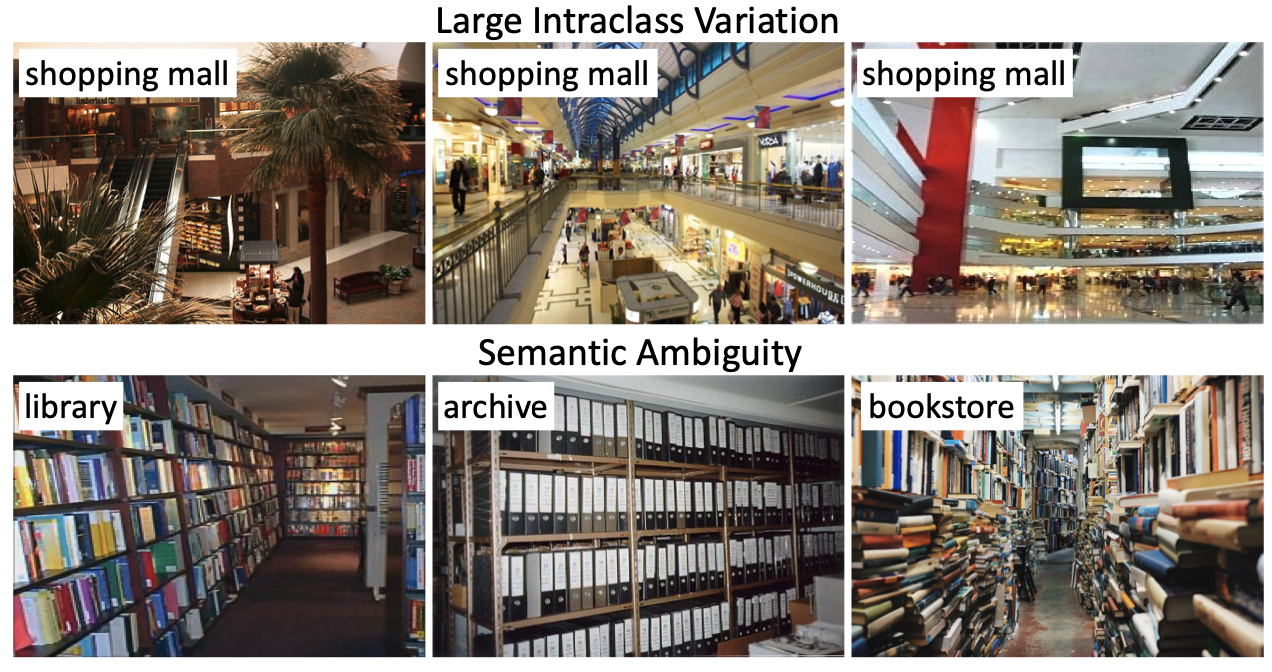
\includegraphics[width=\textwidth]{img/scene_class.png}
    \caption{Problem różnorodności wewnątrzklasowej oraz wieloznaczności semantycznej \cite{zeng2021deep}.}
    \label{fig:scene-class}
\end{figure}

Zadanie klasyfikacji sceny polega na przyporządkowaniu kategorii miejsca, które przedstawia obraz. Istnieje duża różnica między klasyfikacją obrazu a klasyfikacją sceny w kontekście trundości. Klasyfikacja obrazu jako taka zajmuje się przyporządkowaniem klasy obiektu pierwszoplanowego, np. czy na obrazie znajduje się pies, czy kot. Klasyfikacja sceny natomiast musi wziąć pod uwagę wszystkie cechy obrazu, zarówno tła, jak i pierwszego planu, by określić odpowiednie miejsce. 

W kontekście środowisk wewnętrznych klasyfikacja scen stanowi wyzwanie ze względu na zmienność scen wewnętrznych, obecność okluzji oraz fakt, że ten sam typ sceny może wyglądać inaczej na różnych obrazach. Wyróżniamy między innymi problem różnorodności wewnątrz klasowej oraz wieloznaczności semantycznej, co zostało przedstawione na rys. \ref{fig:scene-class}. Pierwszy z nich polega na fakcie, iż jedno miejsce może zostać przedstawione w bardzo różnej konfiguracji m.in. oświetlenia, ekspozycji, obiektów znajdujących się na obrazie. Drugi jest związany z występowaniem tych samych obiektów dla różnych klas scen.

\subsubsection{Segmentacja obrazu}
\begin{figure}[ht!]
    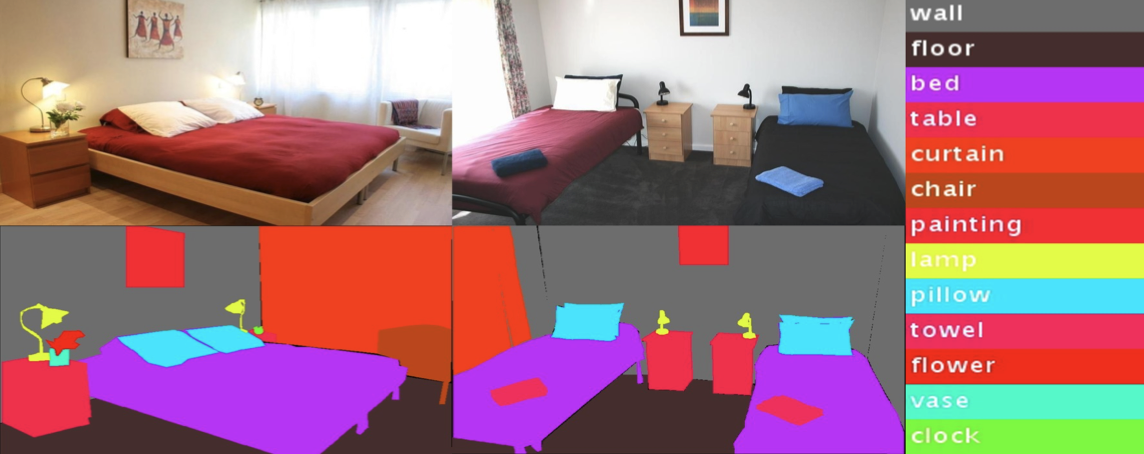
\includegraphics[width=\textwidth]{img/segment.png}
    \caption{Segmentacja wewnątrz pomieszczeń \cite{zhang2018context}.}
    \label{fig:segment}
  \end{figure}
  
Zadanie segmentacji obrazu to przyporządkowanie każdemu pikselowi etykiety takiej jak ,,łóżko'', ,,kanapa'' lub ,,umywalka'', do każdego piksela w obrazie (rys. \ref{fig:segment}). W rezultacie obraz zostaje podzielony na spójne regiony pod względem pewnych własności. Segmentacja może być reprezentowana jako tablica 2D, gdzie każdy element odpowiada pikselowi w obrazie wejściowym i ma wartość wskazującą jego etykietę klasy.

Zadanie segmentacji można rozszerzyć do zadania segmentacji instancji (ang. instance segmentation), czyli segmentacji klasycznej rozszerzonej o rozróżnienie poszczególnych obiektów w ramach tej samej klasy. W przypadku klasycznej wersji nie jesteśmy w stanie rozróżnić dwóch stojących obok siebie łóżek, gdyż mapa segmentacji jest dla nich jednakowa. Segmentacja instancji pozwala natomiast takie rozróżnienie uczynić. Segmentacja semantyczna w dalszej części pracy będzie odnosić się do klasycznej wersji. Segmentacja instancji nie jest tematem pracy.
% # TODO: Zamienić obrazki definicji klasyfikacji i segmentacji na te z mojego zbioru

\subsection{Nadzorowane uczenie maszynowe}

Uczenie maszynowe jest częścią sztucznej inteligencji, które umożliwia przeprowadzanie wnioskowania z danych. Algorytmy te rozpoznają wzorce i dokonują przewidywań.

Uczenie nadzorowane to rodzaj uczenia maszynowego, w którym algorytm jest szkolony na etykietowanym zestawie danych, gdzie pożądane wyjście dla danego wejścia jest już znane. W kontekście głębokiego uczenia się, algorytmy uczenia nadzorowanego wykorzystują sieci neuronowe do uczenia się z danych i dokonywania przewidywań.

Jedną z głównych zalet wykorzystania głębokiego uczenia do uczenia nadzorowanego jest możliwość uczenia się złożonych i nieliniowych zależności wynikających z danych. Głębokie sieci neuronowe, z ich wieloma warstwami, mogą uczyć się i reprezentować wielowymiarowe i abstrakcyjne cechy danych, co pozwala im osiągnąć satysfakcjonujące rezultaty w wielu zadaniach. Co więcej, algorytmy głębokiego uczenia mogą obsługiwać duże ilości danych i mogą być łatwo zrównoleglone, co pozwala na skrócenie czasu treningu.

Istnieją jednak również ograniczenia w stosowaniu głębokiego uczenia do uczenia nadzorowanego. Jednym z ograniczeń jest konieczność posiadania dużej ilości oznaczonych danych. Aby wytrenować głęboką sieć neuronową, wymagana jest ich znaczna ilość. Dane nie zawsze mogą być łatwo dostępne lub łatwe do uzyskania. Co więcej, algorytmy głębokiego uczenia są często podatne na niskie obciążenie lub wysoką wariancję, zwłaszcza gdy ilość i jakość danych jest ograniczona. Może to prowadzić do słabej generalizacji.
\subsection{Głębokie uczenie i konwolucje}
Uczenie głębokie odnosi się do uczenia maszynowego, które charakteryzuje się wykorzystaniem głębokich sieci neuronowych. Składają się one z wielu warstw sztucznych neuronów. W kontekście wizji komputerowej głębokie uczenie jest wykorzystywane do skutecznego rozwiązywania wielu zadań, w tym klasyfikacji obrazów, wykrywania obiektów czy segmentacji semantycznej.

Jedną z kluczowych zalet głębokiego uczenia w wizji komputerowej jest zdolność do automatycznego uczenia się hierarchicznych reprezentacji obrazów. Wykorzystuje je się do wyodrębnienia wysokopoziomowych cech, które są wysoce zróżnicowane dla danego zadania. Stanowi to kontrast do tradycyjnych metod widzenia komputerowego, które zazwyczaj opierają się na ręcznie opracowanych cechach.

\subsection{Rozwój klasyfikacji obrazów}
Jedną z najwcześniejszych i najbardziej wpływowych prac w dziedzinie głębokich splotowych sieci neuronowych (CNN) jest ,,ImageNet Classification with Deep Convolutional Neural Networks'' autorstwa Alexa Krizhevsky'ego et al. (2012)\cite{krizhevsky2017imagenet}. W pracy tej przedstawiono zastosowanie głębokich sieci neuronowych do klasyfikacji obrazów i osiągnięto najwyższe wyniki na zbiorze danych ImageNet. Praca ta wyznaczyła nowy punkt odniesienia dla klasyfikacji obrazów i zapoczątkowała szerokie zastosowanie CNN w zadaniach widzenia komputerowego.

W kolejnych latach wielu badaczy zaproponowało różne modyfikacje i ulepszenia podstawowej architektury CNN. Jednym z ważnych wkładów jest architektura Inception, wprowadzona przez Szegedy et al. w ,,Going Deeper with Convolutions'' (2015)\cite{szegedy2015going}. Architektura Inception wykorzystuje kombinację różnych rozmiarów filtrów konwolucyjnych do ekstrakcji cech w wielu skalach, co pozwala sieci uczyć się bardziej złożonych i abstrakcyjnych cech niż wcześniejsze architektury.

Kolejną ważną innowacją było wykorzystanie połączeń rezydualnych, które zostało zaproponowane przez He et al. w ,,Deep Residual Learning for Image Recognition'' (2016)\cite{he2016deep}. Połączenia rezydualne pozwalają na trenowanie znacznie głębszych sieci, zapobiegając problemowi zanikających gradientów. Tak jak przedtem ImageNet posłużył do wykazania zalet tego rozwiązania.

Podsumowując, głębokie CNN są wysoce efektywne w zadaniach widzenia komputerowego, takich jak klasyfikacja obrazów. Rozwój głębokich CNN zaznaczył się kilkoma ważnymi kamieniami milowymi, takimi jak stosowanie różnych filtrów splotowych oraz wykorzystaniem połączeń rezydualnych. Te innowacje doprowadziły do znacznej poprawy wydajności na zbiorze danych ImageNet i zainspirowały dalsze badania w innych zadaniach widzenia komputerowego.
\subsection{Rozwój segmentacji semantycznej}
Jednym z najwcześniejszych i najbardziej wpływowych artykułów w dziedzinie głębokich CNN do segmentacji semantycznej jest ,,Fully Convolutional Networks for Semantic Segmentation'' autorstwa Longa, Shelhamera i Darrella (2015)\cite{fcn}. W pracy tej, zaprezentowanej na konferencji Computer Vision and Pattern Recognition (CVPR), przedstawiono architekturę sieci w pełni splotową (FCN) do segmentacji semantycznej. Architektura FCN wykorzystuje serię warstw splotowych i upsamplingu do produkcji gęstych predykcji per-piksel. Praca ta pokazała, że CNN mogą być wykorzystane do predykcji na poziomie pikseli i stworzyła podstawy dla wielu późniejszych podejść do segmentacji semantycznej.

Innym kluczowym wkładem w dziedzinie segmentacji semantycznej jest ,,U-Net: Convolutional Networks for Biomedical Image Segmentation'' autorstwa Ronneberger, Fischer i Brox (2015)\cite{ronneberger2015u}. W pracy tej, zaprezentowanej na międzynarodowej konferencji Medical Image Computing and Computer-Assisted Intervention (MICCAI), przedstawiono architekturę U-Net do segmentacji obrazów biomedycznych. Architektura U-Net wykorzystuje kombinację warstw splotowych i poolingowych do ekstrakcji cech w wielu skalach oraz serię warstw upsamplingu do produkcji gęstych predykcji per-piksel. Praca ta pokazała, że architektura U-Net dzięki zastosowaniu połączeń pomijających (skipping connections) jest w stanie znacznie lepiej rekonstruować obraz. Szczególnie dotyczy to elementów małej skali, które wcześniej były pomijane przez FCN. Praca ta została szeroko wykorzystana w obrazowaniu medycznym i nie tylko.

Kolejną ważną pracą w dziedzinie segmentacji semantycznej jest ,,DeepLab: Semantic Image Segmentation with Deep Convolutional Nets, Atrous Convolution, and Fully Connected CRFs'' autorstwa Chen, Papandreou, Kokkinos, Murphy i Yuille (2016)\cite{deeplab}. W pracy tej, zaprezentowanej na International Conference on Computer Vision (ICCV), przedstawiono architekturę DeepLab do segmentacji semantycznej. Architektura DeepLab wykorzystuje rozszerzony splot (atrous convolution) do zwiększenia pola widzenia warstw splotowych oraz warunkowe pola losowe (CRF) do dopracowania predykcji. Praca ta pokazała, że użycie rozszerzonego splotu i CRF może poprawić efekty segmentacji semantycznej.

Podsumowując, segmentacja semantyczna jest zadaniem o dużym znaczeniu w wizji komputerowej, a głębokie CNN okazały się wysoce skuteczne w rozwiązywaniu tego zadania. Rozwój głębokich CNN do segmentacji semantycznej został oznaczony przez kilka ważnych kamieni milowych, w tym wprowadzenie FCN przez Long et al., U-Net przez Ronneberger et al. i DeepLab przez Chen et al. Te architektury wyznaczyły nowe standardy w segmentacji semantycznej i zostały szeroko przyjęte w różnych dziedzinach zastosowań.




\subsection{DeepLabV3}
Literatura uważa go za model lepszy od sieci U-Net czy FCN. Model DeepLabV3 (rys. \ref{fig:deeplabv3}) nie korzysta z połączeń pomijających. Informacje o kontekście w wielu skalach uzyskuje przez moduł Spatial Pyramid Pooling (SPP). Wykorzystuje on bloki Atrous Spatial Pyramid Pooling (ASPP) oraz klasyczny pooling. Bloki ASPP składają się ze splotu, normalizacji pakietowej oraz funkcji aktywacji ReLU. Sploty przyjmują różną postać. Pierwszy blok to splot o jądrze 1x1. Następne bloki korzystają z rozszerzonego splotu o dylatacji oraz wypełnieniu (padding) równemu współczynnikowi rozszerzenia (dilatation rate). Dla kolejnych 3 bloków wynosi on 12, 24, 36. Ostatni blok SPP to zwykły pooling. Bloki składające się na moduł SPP są następnie dodawane wzdłużnie i poddawane splotowi. Następnie egzekwuje się splot o wyjściowej liczbie kanałów równej ilości klas. Końcowy etap obejmuje upsampling do pożądanego wymiaru.
\begin{figure}[ht!]
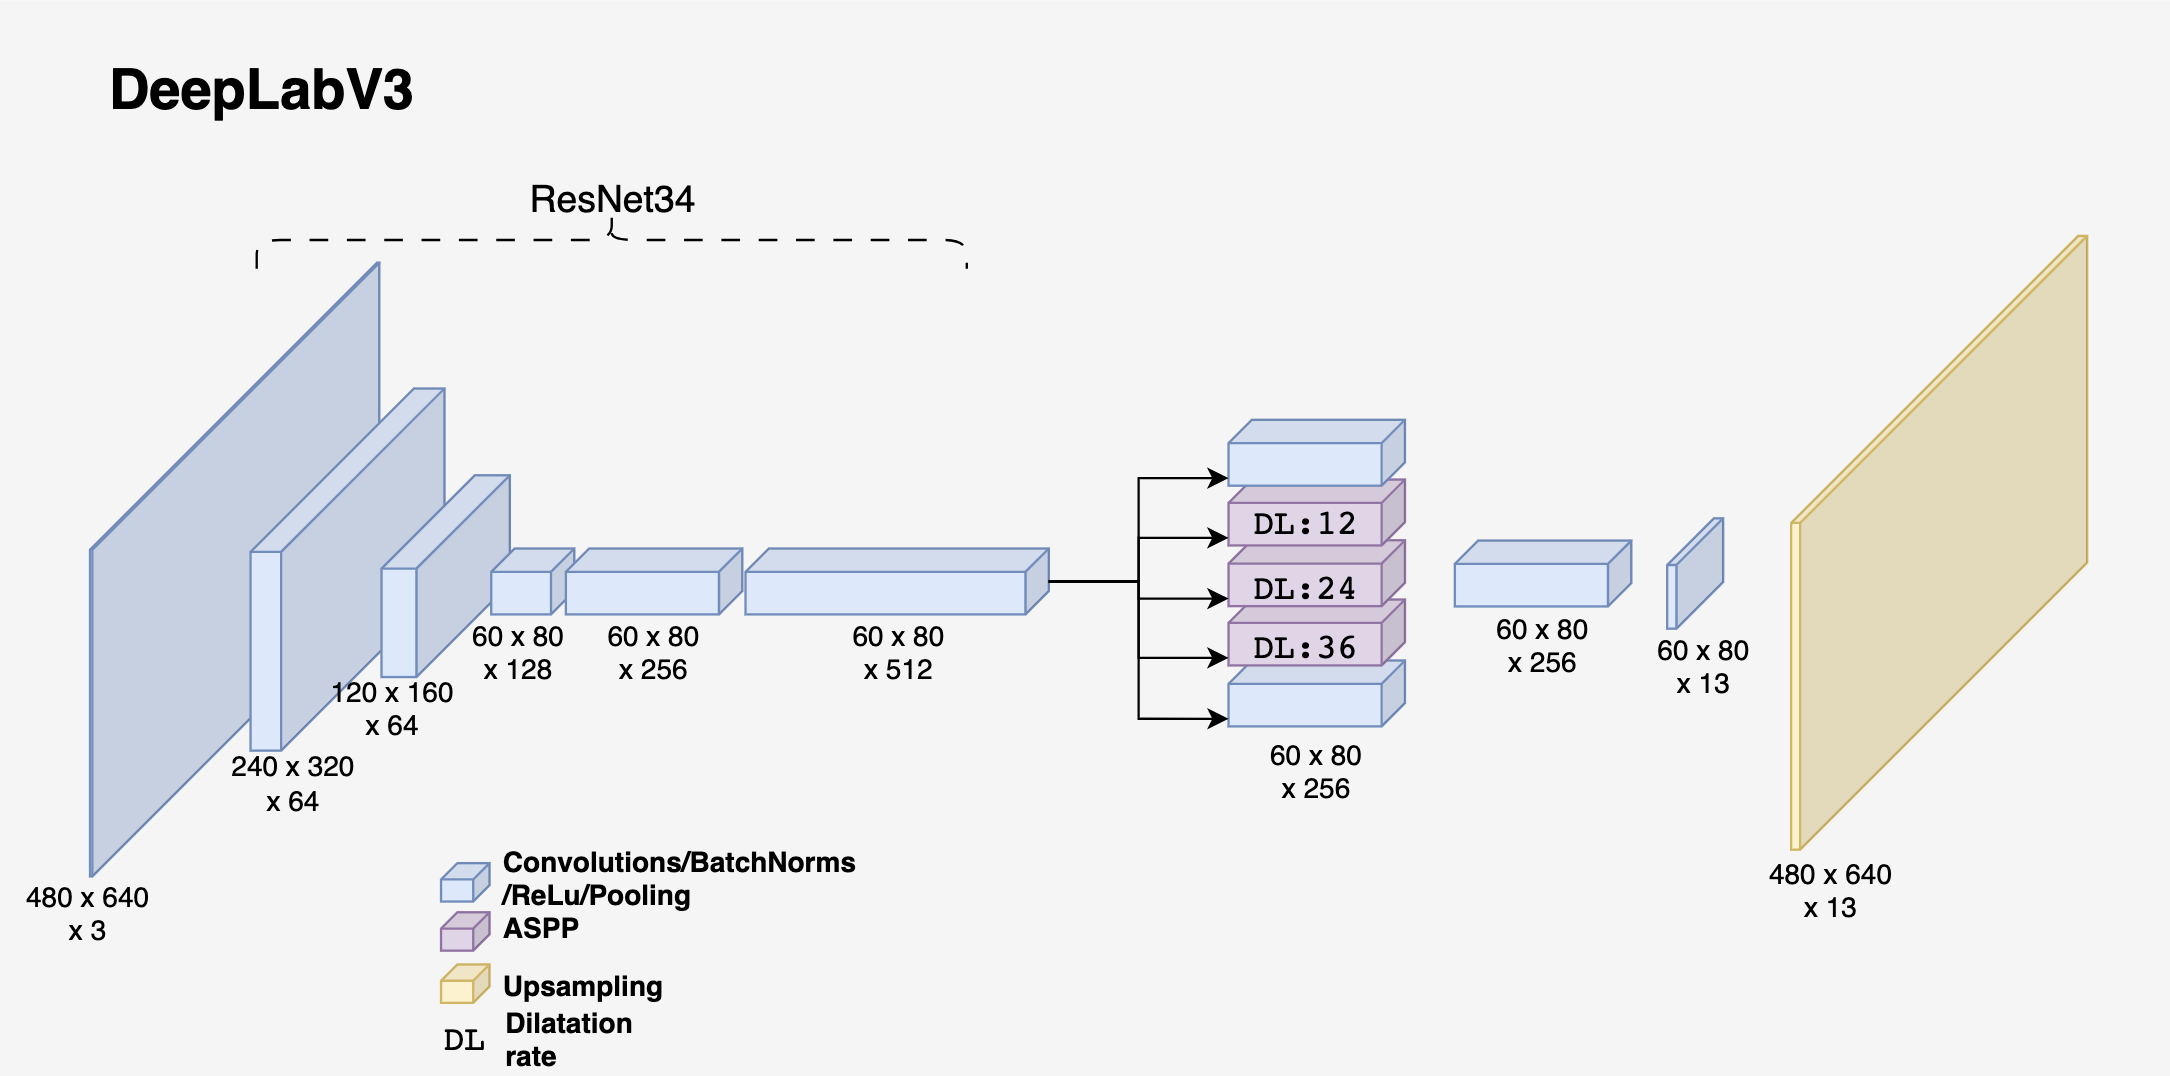
\includegraphics[width=\textwidth]{deeplabv3-new.png}
\caption{Klasyczna architektura DeepLabV3 z backbonem ResNet34.}
\label{fig:deeplabv3}
\end{figure}


% \subsection{DeepLabV3}
% Literatura uważa go za model lepszy od sieci U-Net czy FCN. Model DeepLabV3 (rys. \ref{fig:deeplabv3}) nie korzysta z połączeń pomijających. Informacje o kontekście w wielu skalach uzyskuje przez moduł Spatial Pyramid Pooling (SPP). Wykorzystuje on bloki Atrous Spatial Pyramid Pooling (ASPP) oraz klasyczny pooling. Bloki ASPP składają się ze splotu, normalizacji pakietowej oraz funkcji aktywacji ReLU. Sploty przyjmują różną postać. Pierwszy blok to splot o jądrze 1x1. Następne bloki korzystają z rozszerzonego splotu o dylatacji oraz wypełnieniu (padding) równemu współczynnikowi rozszerzenia (dilatation rate). Dla kolejnych 3 bloków wynosi on 12, 24, 36. Ostatni blok SPP to zwykły pooling. Bloki składające się na moduł SPP są następnie dodawane wzdłużnie i poddawane splotowi. Następnie egzekwuje się splot o wyjściowej liczbie kanałów równej ilości klas. Końcowy etap obejmuje upsampling do pożądanego wymiaru.
% \begin{figure}[ht!]
% 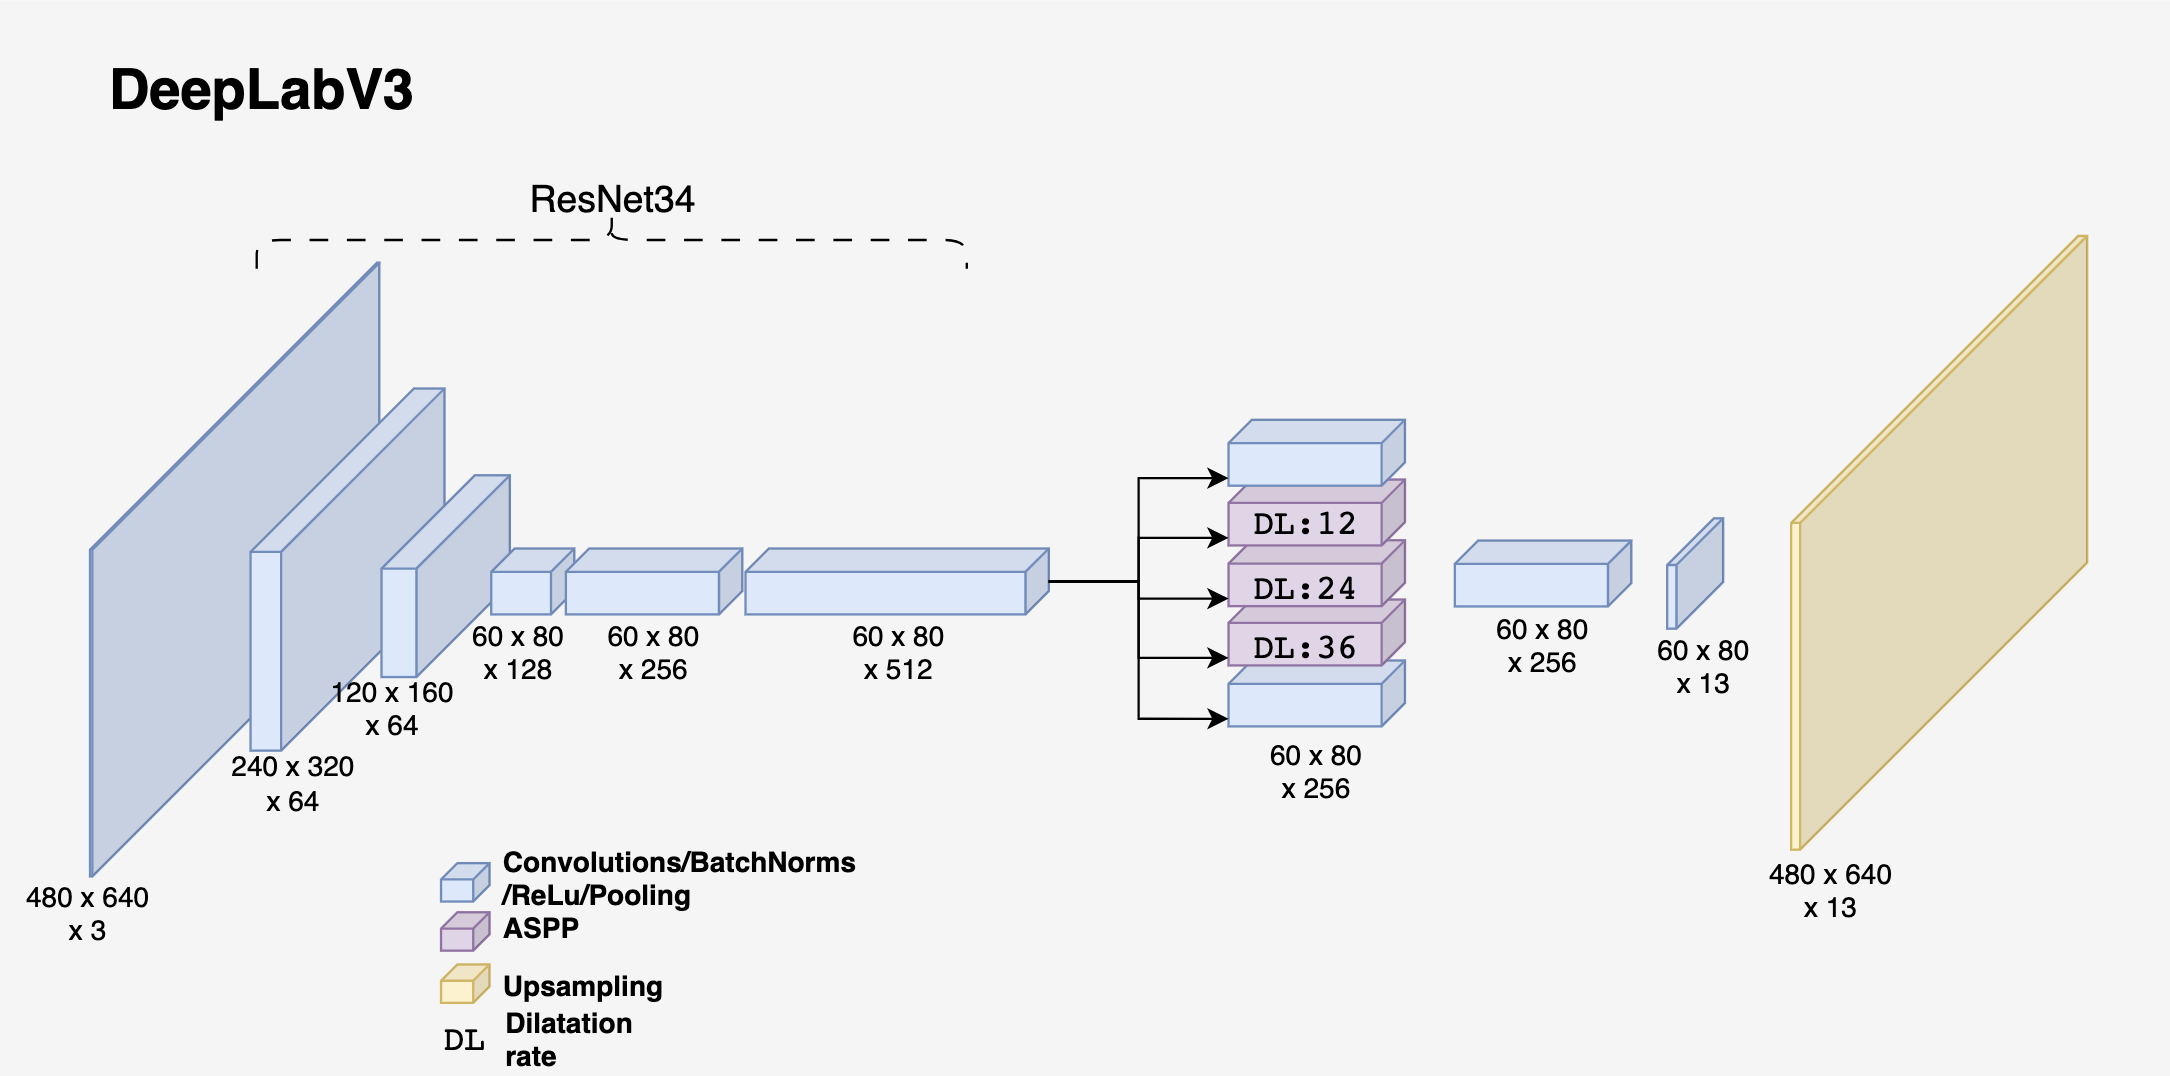
\includegraphics[width=\textwidth]{deeplabv3-new.png}
% \caption{Klasyczna architektura DeepLabV3 z backbonem ResNet34.}
% \label{fig:deeplabv3}
% \end{figure}

\subsection{Finetuning}
Finetuning jest metodą uczenia głębokich sieci neuronowych. Polega on na odtworzeniu wag modelu, wcześniej wytrenowanego na dużym zbiorze danych jak ImageNet, a następnie próbie dostosowania go do obecnie rozważanego problemu. W kontekście wizji komputerowej pierwsze warstwy modelu są najczęściej ogólne i odnoszą się do generalnych cech obrazu. Ta wiedza pozwala wnioskować, że pierwsza część modelu nie zależy w głównej mierze od zbioru danych oraz rozważanego zadania, tylko jest czymś ogólnym dla wielu problemów przetwarzania obrazu. Zatem pojawia się możliwość ponownego użycia część gotowego modelu. W takim przypadku mowa o transferze wiedzy. Technicznie finetuning najczęściej rozpoczyna się od uczenia modelu, wykorzystując jedynie ostatnie warstwy. W miarę kolejnych epizodów uczenia wykorzystuje się coraz więcej warstw sieci. Taki zabieg nazwy się odmrażaniem kolejnych warstw sieci.
\subsection{Uczenie wielozadaniowe}
Uczenie wielozadaniowe jest techniką uczenia maszynowego, w której model jest trenowany do wykonywania wielu zadań jednocześnie. Zabieg ten stosuje się w celu nauczenia się wspólnych reprezentacji, które mogą poprawić skuteczność we wszystkich zadaniach. To podejście zyskało uwagę w ostatnich latach ze względu na rosnące zapotrzebowanie na modele, które mogą wykonywać wiele zadań z wysoką dokładnością i wydajnością. Uczenie wielozadaniowe ma szereg zastosowań, takich jak widzenie komputerowe, przetwarzanie języka naturalnego i rozpoznawanie mowy.

Sebastian Ruder w swoim przeglądzie literatury ,,An Overview of Multi-Task Learning in Deep Neural Networks'' (2017) \cite{ruder2017overview} dość zwięźle definiuje uczenie wielozadaniowe jako optymalizację co najmniej dwóch funkcji straty. Co więcej, pokazuje, że takie podejście ma swoje silne biologiczne analogie. Autor dopatruje się tutaj odpowiedzi na pytanie, czym jest uczenie się uczenia (learnig to learn), a więc główna przesłanka bardzo silnego nurtu meta-learningu. Podkreśla, że uczenie wielozadaniowe pomaga osiągać lepsze rezultaty niż klasyczne uczenie jednego zadnia. Zachęca nawet do stosowania uczenia wielozadaniowego w przypadku, gdy potrzebujemy zaledwie jednego zadania poprzez znalezienie zadania lub zadań komplementarnych. Autor wielokrotnie odwołuje się do dzieła ,,Multitask learning: A knowledge-based source of inductive bias'' (1993) \cite{caruana1993multitask} przypominając, że uczenie wielozadaniowe przyczynia się do lepszej generalizacji modelu, a więc uniezależnienie się od domeny uczącej na rzecz szeroko pojętej wiedzy.

Ruder opisuje dwa główne podejścia do uczenia wielozadaniowego — twarde oraz miękkie dzielenie wag sieci (soft/hard parameter sharing). Twarde dzielenie wag jest najczęściej stosowane. Polega na uwspólnieniu pierwszej części sieci, odpowiedzialnej za zdefiniowanie przestrzeni reprezentacji (ang. backbone) oraz rozdzieleniu kolejnych warstw związanych z konkretnym zadaniem. Miękkie dzielenie wag polega na zbudowaniu wielu sieci, odpowiednich dla danego zadania. Co więcej, sieci te podczas uczenia są regularyzowane w ten sposób, aby zachęcić je do posiadania jak najpodobniejszych wag.

Takie podejście może się powieść jedynie w przypadku, kiedy dwa zadania są powiązane ze sobą. Powstało wiele prac poświęconych odpowiedzi na pytanie, które zadania warto wybrać, a które należy rozpatrywać osobno. Jednym z takich dzieł jest praca zespołu ze Stanfordu ,,Which Tasks Should Be Learned Together in Multi-task Learning?'' Standley et al. (2020) \cite{standley2020tasks}. Przedstawia ona pojęcie negatywnego wpływu (ang. negative transfer), który najprościej rzecz ujmując sprawia, że sieć uczy się gorzej niż pojedyncze sieci. Autorzy zbadali, że największy wpływ na jakość uczenia wielozadaniowego ma właśnie odpowiedni dobór zadań, a niekoniecznie rozmiar zbioru danych czy wielkość modelu. Oczywiście należy zwrócić uwagę, że przytoczone czynniki nie są bez znaczenia, jedynie w porównaniu z doborem zadań mają pomijalne znaczenie. Co ciekawe zadania afiniczne względem siebie mogą mieć dodatni wpływ w przypadku transferu wiedzy, a nie muszą być afiniczne w kontekście uczenia wielozadaniowego.

Gdy jednak zadania są pokrewne względem siebie, jesteśmy w stanie zaobserwować konkretne korzyści związane ze wspólnym uczeniem. Ruder wymienia kilka najważniejszych. Po pierwsze zyskujemy tak zwaną niejawną augmentację danych (ang. implicit data augmentation). Każde z zadań posiada pewien szum związany z konkretnym zadaniem. Uczenie wielu zadań pozwala w pewnym stopniu wyeliminować szum związany z konkretnym zadaniem na rzecz lepszej generalizacji. Kolejną zaletą jest lepsze skupienie uwagi na ważnych informacjach. Ma to szczególne znaczenie w przypadku gdy dane są ograniczone lub wielowymiarowe. Uczenie wielozadaniowe może pomóc w wyborze tych najbardziej znaczących cech. Co więcej, wspólna wiedza zdobyta podczas uczenia może okazać się znacząca. Niektóre cechy są łatwiejsze do wykrycia dla jednego zadania, inne dla drugiego. Łącząc te informacje przez tak zwane ,,podsłuchiwanie'' (ang. eavesdropping) model jest w stanie zbudować lepszą przestrzeń reprezentacji. Oprócz zyskania na jakości modelu przypadek twardego dzielenia wag pozwala znacząco ograniczyć wielkość modelu. Nie trzeba bowiem stosować wielu backbone'ów, które stanowią największą część modelu w kontekście liczby parametrów. Implikuje to znacznie zmniejszenie czasu uczenia oraz wnioskowania \cite{standley2020tasks}.